\section{\model{}: Steering Vision Transformers with Text}
\label{sec:method}

% method text-conditioned visual
% architecture modifications
% datasets + training signals
% inference-time text conditioning (jona)
% experiments (hypothesis validating) ## arxiv - before method
% conditional retrieval kNN
% baseline: late fusion
% without losing classification
% pareto explain
% attention does steer to text descriptions (results by segmentation)
% analysis / applications
% personalized: how to condition (PODS)
% anomaly detection 
% where are my keys (?)
% (???) hallucination detection, negation 
% (???) VQA
% ablations / features of our approach -- justifying choices of method (a subset of task)
% architecture (sigmoid gating, FFN block, CA blocks)
% backbones (MAE, SigLIP) (?)
% scale the model (ViT-L)
% losses (?)
% resolution (?)
% token length [optional!]
% conclusion

% \MT{skipping for now as discussed with MG}


Next, we describe the architectural modifications and post-training to turn a pretrained ViT into a \model{} model.
% We inject text into a frozen ViT through gated cross-attention layers that steer visual features towards the text prompt without degrading them.
% We describe \model{}'s architectural modifications and training data and objectives below.

% As illustrated in \cref{fig:arch_training}, our architecture consists of three components:
% (1)~a frozen text encoder (RoBERTa-Large~\cite{liu2019roberta}) that produces token-level embeddings from the input prompt;
% (2)~a lightweight multimodal adapter (MLP) that projects these text embeddings into the visual embedding space; and
% (3)~tanh-gated cross-attention layers interleaved within a frozen ViT that progressively fuse textual cues into the visual representation.
% Given an image and a text prompt, SHIFT produces text-contextualized patch-level visual features that remain in the base ViT's embedding space.
% We train the model on a diverse mixture of referential segmentation datasets (Section~\ref{sec:data}) using a binary segmentation objective at the ViT patch level (Section~\ref{sec:objective}).
% The segmentation head serves solely as a training signal and is discarded at inference; the output of interest is the steered visual representation itself.

\subsection{Architecture}
\label{sec:arch}

\begin{wrapfigure}{r}{0.4\textwidth}
\centering
\vspace{-15mm}
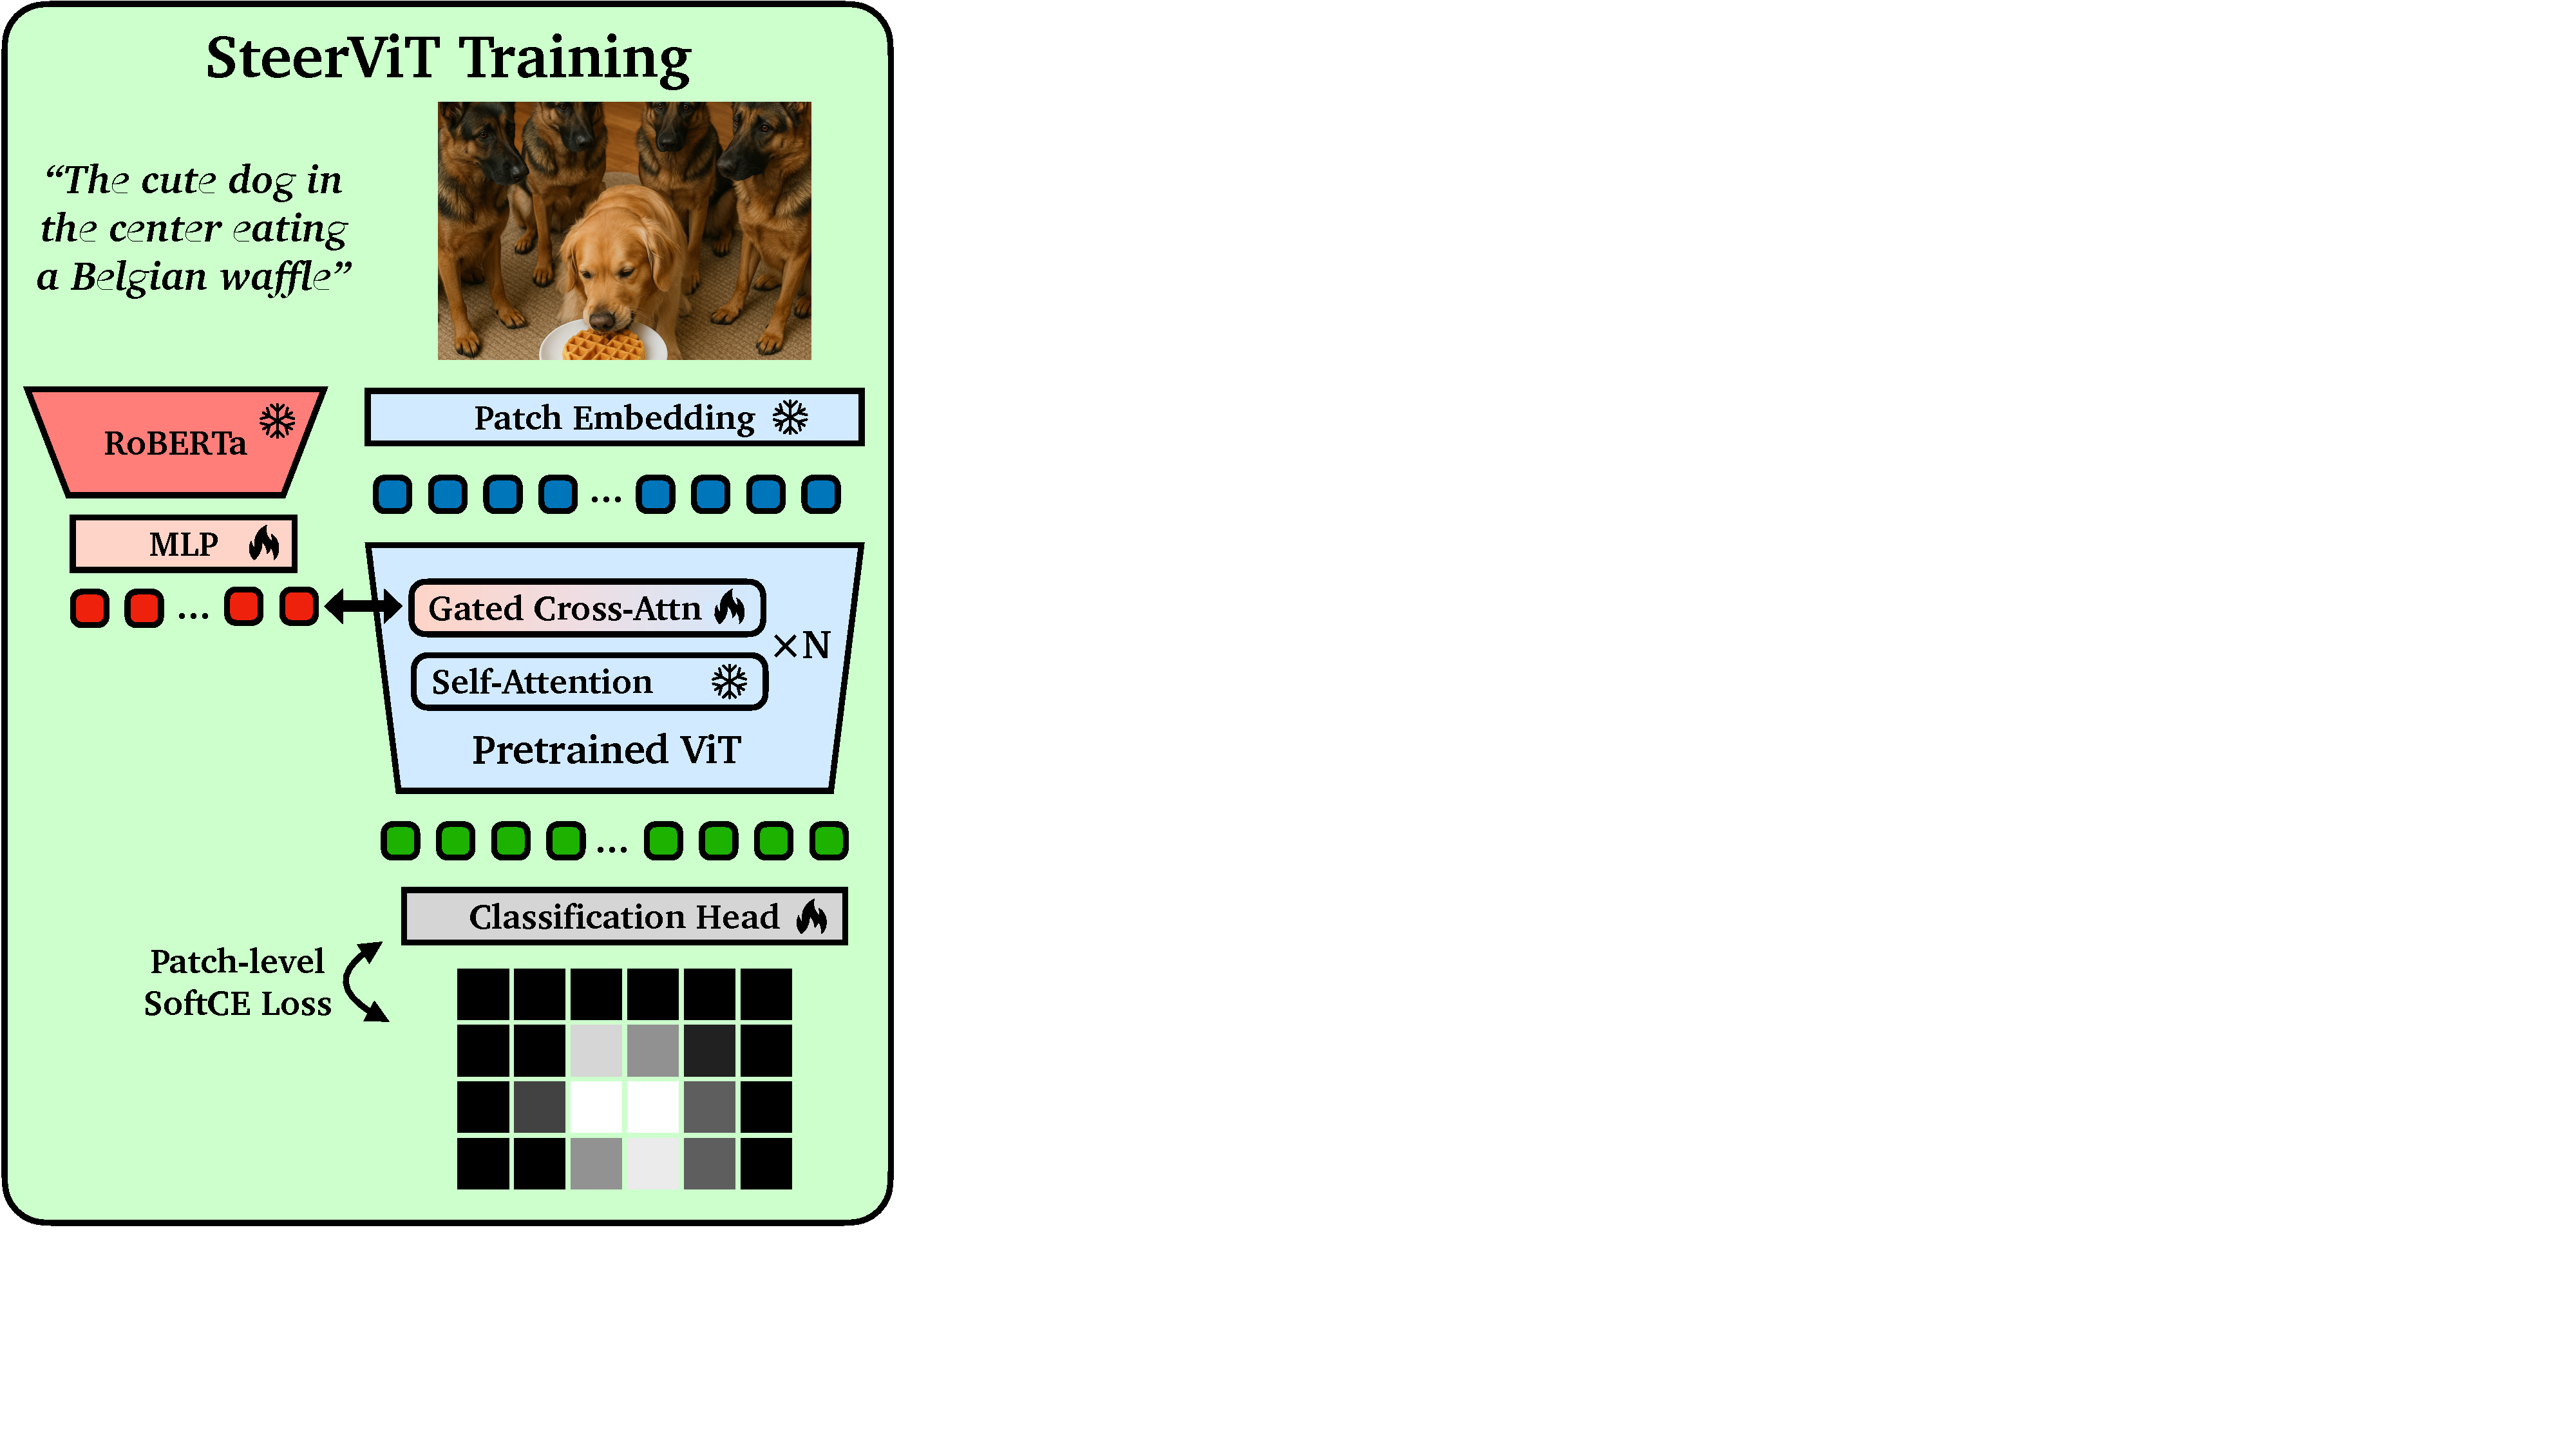
\includegraphics[width=\linewidth]{figures/training_architecture.pdf}
\vspace{-3mm}
\caption{\textbf{Steering any ViT using text conditioning.}
Our method adds lightweight vision-to-language cross-attention layers within pretrained ViT blocks and applies a patch-level segmentation proxy objective to fuse prompt cues into patch tokens. We train on XXXX \YA{add:We train this with existing referential object localisation datasets of X~M images??}
\YA{great job! maybe all RoBERTa-"L"? or "M"? and also add somewhere "pretrained ViT"? }
}
\label{fig:arch_training}
\end{wrapfigure}

As illustrated in \cref{fig:arch_training}, our \model{} consists of four components:

\colorbox{visionblue}{\textbf{A. Visual encoder.}}
For an image $X_v \in \mathbb{R}^{H \times W \times 3}$, a ViT produces a sequence of $N$ patch tokens $Z_v \in \mathbb{R}^{N \times d_v}$ and optionally a  \texttt{[CLS]} token, where $d_v$ is the embedding dimension.
All original ViT parameters remain frozen throughout training; new capacity enters exclusively through the interleaved cross-attention layers described below.
While most experiments adopt the DINOv2 ViT-B/14~\cite{oquab2024dinov2} as our backbone, we will show that our approach also improves steerability of SigLIP or MAE.


\colorbox[RGB]{234,133,125}{\textbf{B. Text encoder.}}
We adopt a frozen, pretrained text encoder (RoBERTa-Large~\cite{liu2019roberta}) to produce token-level embeddings $Z_t \in \mathbb{R}^{L \times d_t}$ for a given input conditioning prompt $X_t$, where $L$ is a variable number of text tokens and $d_t$ is the text embedding dimension.
% Given an input prompt $X_t$, the encoder extracts a variable-length sequence of token embeddings $Z_t \in \mathbb{R}^{L \times d_t}$, where $L$ is the number of text tokens and $d_t$ is the text embedding dimension.
% We $\ell_2$-normalize these embeddings before passing them to the multimodal adapter.

\colorbox{textred}{\textbf{C. Multimodal adapter.}}
Each language embedding $Z_t^i$ is $\ell_2$-normalized and fed through a trainable two-layer MLP that projects the sequence into visual-aligned tokens $H_t \in \mathbb{R}^{L \times d_v}$.
We add learnable positional encoding to $H_t$ to preserve token order before injecting them into the ViT through the gated cross-attention mechanism. 
\YA{I think it wouldn't hurt to describe the steps you're doing with math.. including actually the L2 normalisation earlier etc. }



\tikz[baseline=(X.base)] 
\node[rectangle,
      inner sep=2pt,
      outer sep=0pt,
      shade,
      left color=textred,
      right color=visionblue] (X)
{\textbf{D. Gated cross-attention layers.}}; % <-- DON'T remove - Semicolon needed to tikz to compile without error
To fuse textual conditioning into the ViT's residual stream, we invert the gated cross-attention (CA) formulation from Flamingo~\cite{alayrac2022flamingo} by allowing hidden vision states to attend to language tokens (language-to-vision CA in \cite{alayrac2022flamingo}).
We insert CA layers into every other Transformer encoder block (e.g., 6 CA layers across 12 blocks in ViT-B), with each layer consisting of multi-head cross-attention followed by a feed-forward network (FFN).
% To fuse textual conditioning into the ViT's residual stream, we adapt the gated cross-attention (CA) dense formulation from Flamingo~\cite{alayrac2022flamingo} \YA{, but essentially apply it in a reverse manner: we let the vision model look at text-features, not the other way around. (something like this)}.
% Each inserted layer applies multi-head cross-attention followed by a feed-forward network (FFN).
The visual patch tokens $Z_v^{(\ell)}$ at layer $\ell$ serve as queries and the adapted text tokens $H_t$ serve as keys and values:
\begin{equation}
\small
\hat{Z}_v^{(\ell)} = \text{CA}(Z_v^{(\ell)}, H_t) = \text{softmax}\!\left(\frac{Q K^\top}{\sqrt{d_k}}\right) V, \quad Q = Z_v^{(\ell)} W_Q, \; K = H_t W_K, \; V = H_t W_V \, .
\end{equation}
The output is integrated into the residual stream through a tanh gate with a layer-specific learnable scalar $\alpha_\ell$, initialized to zero:
\begin{equation}
Z_v^{(\ell+1)} = Z_v^{(\ell)} + \tanh(\alpha_\ell) \cdot \text{FFN}\!\left(\hat{Z}_v^{(\ell)}\right).
\label{eq:gated_ca}
\end{equation}
Since $\tanh(0) = 0$, the model is mathematically identical to the frozen ViT at initialization.
% As training progresses, the gates learn to open, allowing the model to smoothly incorporate text conditioning. 
Despite the zero-initialisation, the gate still receives a learning signal since
\begin{equation}
\frac{\partial Z_v^{(\ell+1)}}{\partial \alpha_\ell}
=
\mathrm{sech}^2(\alpha_\ell)\,\mathrm{FFN}\!\left(\hat{Z}_v^{(\ell)}\right),
\end{equation}
and $\mathrm{sech}^2(0)=1$. %, yielding \( \left.\frac{\partial Z_v^{(\ell+1)}}{\partial\alpha_\ell}\right|_{\alpha_\ell=0} = \mathrm{FFN}(\hat{Z}_v^{(\ell)}).\)
Thus, $\alpha_\ell$ can move away from zero during optimization, gradually activating the conditioning pathway and allowing the model to incorporate language-based clues.

\subsection{Training Objective}
\label{sec:objective}
In order to encourage the vision encoder to leverage and incorporate language clues, we design a pretext task requiring consideration of the prompt to be solved. We select referential segmentation for this purpose, where, given an image $X_v$ and a prompt $X_t$ referring to a target object, the model predicts which patches correspond to the referred object.


The ground-truth is given by the fraction of foreground pixels within of a pixel-wise binary segmentation mask that was patchified to match the ViT's $n \times n$ grid of non-overlapping patches.
% The ViT partitions the image into an 
% We convert the ground-truth binary segmentation mask $M \in \{0, 1\}^{H \times W}$ into patch-level labels $y \in [0, 1]^{n \times n}$ by computing the fraction of foreground pixels within each patch.
A linear classifier head maps each patch representation $Z_v^i \in \mathbb{R}^{d}$ to a probability $p_i$ through softmax.
We adopt the soft cross-entropy loss
\begin{equation}
\mathcal{L} = - \sum_{i=1}^{n \times n} y_i \log p_i \, ,
\label{eq:loss}
\end{equation}
% We optimize the network with a binary cross-entropy loss over all patches:
% \begin{equation}
% \mathcal{L} = -\frac{1}{n^2} \sum_{i=1}^{n^2} \left[ \hat{y}_i \log \sigma(p_i) + (1 - \hat{y}_i) \log (1 - \sigma(p_i)) \right],
% \label{eq:loss}
% \end{equation}
% where $\sigma$ denotes the sigmoid function.
as it encourages the CA layers to route
% task-relevant
textual information into the corresponding visual patch tokens, producing steered representations.
% as a byproduct.
Performing segmentation on a patch- rather than pixel-level reduces the training complexity and forgoes the need for pixel-level decoders. 


\subsection{Training Data}
\label{sec:data}

We train on a mixture of referential segmentation and grounding datasets to ensure diversity in both visual domains and textual expression styles:

\textbf{RefCOCO, RefCOCO+, RefCOCOg}~\cite{kazemzadeh2014referitgame, yu2016refcocog} provide referring expressions grounded in COCO images.
RefCOCO+ excludes spatial language (e.g., ``left of''), encouraging the model to rely on appearance cues, while RefCOCOg contains longer, more descriptive expressions that exercise the model's capacity for detailed textual understanding.

\textbf{Visual Genome}~\cite{krishna2017visual} (preprocessed following MDeTr~\cite{kamath2021mdetr}) contributes region descriptions paired with bounding boxes across densely annotated scenes.
These descriptions span a broader vocabulary and more complex spatial relationships than the RefCOCO family, increasing the diversity of text conditioning signals.
We use SAM2 to convert bounding boxes to binary segmentation masks.

\textbf{Mapillary Vistas}~\cite{neuhold2017mapillary} provides street-level imagery with fine-grained panoptic annotations.
Including this dataset expands the visual domain beyond COCO's indoor and object-centric bias toward outdoor, driving, and urban scenes, improving out-of-distribution generalization. We use Describe Anything's synthetically generated referential expressions along with accompanying binary segmentation masks. 

This combination \YA{overall X million images and Y annotations} exposes the model to varied scene complexities (from single objects to dense urban panoramas), expression lengths (from two-word labels to multi-sentence descriptions), and visual domains (indoor, outdoor, street-level), encouraging robust text-conditioned representations.
\YA{in expeirments, you should describe training batch size, iterations count, resolution, GPU hours}

\YA{I think we need one more subsection in Section 3 about "Measuring Text-steerability of vision representations" where we describe the task/benchmarks}